\newtheorem{definition}{Definition}[section]
\newtheorem{proposition}{Proposition}[section]
%\theoremstyle{definition} % use not italic font for the rest
%\newtheorem{example}{Example}[section]
\newtheorem{remark}{Remark}[section]

%\DefineVerbatimEnvironment{code}{Verbatim}{frame=single,rulecolor=\color{blue}}
\newcommand{\mathbfx}[1]{{\mbox{\boldmath $#1$}}}
%\newcommand{\R}{{\mathbb R}}
\renewcommand{\P}{{\mathbb P}}
\renewcommand{\H}{{\mathbb H}}
\newcommand{\xxi}{\mathbfx{\xi}}
\newcommand{\xxx}{\mathbf{x}}
\newcommand{\eee}{\mathbf{e}}
\newcommand{\GG}{\mathbf{G}}
\newcommand{\kentc}[1]{\marginpar{\tiny KAM: #1}}
\newcommand{\rckc}[1]{\marginpar{\tiny RCK: #1}}

\fenicschapter{Constructing general reference finite elements}
              {Constructing general reference finite elements}
              {Robert C. Kirby and Kent-Andre Mardal}
              {kirby-1}

%\begin{document}

%\maketitle
%\vspace{-0.3cm}

%\thispagestyle{empty}

\section{Introduction}
The finite element literature contains a huge collection of
approximating spaces and degrees of freedom, many of which are
surveyed in Chapter~\ref{??}, 
Some applications, such as Cahn-Hilliard and
other fourth-order problems, can benefit from very smooth finite
element bases.  While porous media flow requires
vector fields discretized by piecewise polynomial functions with
normal components continuous across cell boundaries.  Many problems in 
electromagnetism call for the tangentially continuous vector fields obtained
by using Nedelec elements~\cite{nedelec}.  Many elements are carefully designed
to satisfy the \emph{inf-sup} condition~\cite{BrezziFortin,g-r},
originally developed to explain stability of discretizations of 
incompressible flow problems.  Additionally, some problems call for low-order
discretizations, while others are effectively solved with high-order
polynomials. 

While the automatic generation of computer programs for finite element
methods requires one to confront the panoply of  finite
element families found in the literature, it also provides a pathway
for wider employment of Raviart-Thomas, Nedelec, and other
difficult-to-program elements.  
Ideally, one would like to
describe the diverse finite element spaces at an abstract level,
whence a computer code discerns how to evaluate and differentiate
their basis functions.  Such goals are in large part accomplished by
the FIAT and SyFi projects, whose implementations are described in
later chapters.  

Projects like FIAT and SyFi may ultimately remain 
mysterious to the end user of a
finite element system, as 
interactions with finite element bases are typically mediated through
tools that construct the global finite element operators.
The end user will typically be satisfied if two conditiones are met. 
First, a finite element system 
should support the common elements used in the application
area of interest.  Second, it should provide flexibility with respect
to order of approximation.

It is entirely possible to satisfy many users by \emph{a priori}
enumerating a list of finite elements and implement only those.  At certain times, this
would even seem ideal.  For example, after the rash of research 
that led to elements such as the Raviart-Thomas-Nedelec and
Brezzi-Douglas-Marini families, development of new families slowed
considerably.  Then, more recent work of lead forth by  Arnold, Falk, and Winther in the context of exterior
calculus has not only led to 
improved understanding of existing element families, but has also
brought a new wave of elements with improved proprerties.  A
generative system for finite element bases can far more
readily assimilate these and future developments.  
Automation also provides generality with respect to the order of approximation that standard libraries
might not otherwise provide. Finally, the end-user might even easilly define his own new element
and test its numerical properties before analyzing it mathematically.  


In the present chapter, we describe the mathematical formulation
underlying such projects as FIAT~\cite{www:fiat,fiat:toms1,fiat:toms2}, 
SyFi~\cite{www:syfi,toms:syfi} and Exterior~\cite{www:exterior}.
This formulation starts from definitions of finite elements as
given classically by Ciarlet~\cite{Ciarlet}.  It then uses basic linear
algebra to construct the appropriate nodal basis for an abstract
finite element in terms of polynomials that are easy to implement and
well-behaved in floating point arithmetic.  We focus on
constructing nodal bases for a single, fixed reference element.  As we
will see in Chapter~\ref{}, form compilers such as
\texttt{ffc}~\cite{www:ffc} and \texttt{sfc}~\cite{www:sfc} will work
in terms of this single reference element.   


Other approaches exist in the literature, such as the hierarchical
bases studied by Szabo and Babuska~\cite{SzaBab91} and extended to \(
H(\mathrm{curl}) \) and \( H(\mathrm{div}) \) spaces in work such
as~\cite{AinCoy02}.  These can provide greater flexibility for
refining the mesh and polynomial degree in finite element methods, but
they also require more care during assembly and are typically constructed
on a case-by-case basis for each element family.  When they are
available, they may be cheaper to construct than using the technique
studied here, but this present technique is easier to apply to an
``arbitrary'' finite element and so is considered in the context of
automatic software.


\section{Preliminaries}
Both FIAT and SyFi work a slightly modified version of the  abstract definition of a finite element introduced by
Ciarlet~\cite{Ciarlet}.
\begin{definition}[A Finite Element]
\label{def:finite:element}
A finite element is a triple \( (K,P,N) \) with
\begin{enumerate}
\item \( K \subset \mathbb{R}^d \) a bounded domain with piecewise
  smooth boundary.  
\item A finite-dimensional space \( P \) of \( BC^m(K,V) \), where \(
  V \) is some normed vector space and \( BC^m \) is the space of
  \( m \)-times bounded and continuosly differentiable functions from
  \( K \) into \( V \).  
\item A dual basis for \( P \), written \( N = \left\{ L_i
    \right\}_{i=1}^{\dim P} \).  These are bounded linear functionals in
    \( ( BC^m(K,V) )^\prime \) and frequently called the \emph{nodes}
    or \emph{degrees of freedom}.
\end{enumerate}
\end{definition}

In this definition, the term ``finite element'' refers not only to
a particular cell in a  mesh, but also to the associated function
space and degrees of freedom.  Typically, the domain \( K \) is some
simple polygonal or polyhedral shape and the function space \( P \)
consists of polynomials.  

Given a finite element, a concrete 
basis, often called the nodal basis, 
for this element can be computed by using the following defintion.  

%The function space \( P \)
%typically consists of polynomials.  Also, this definition is
%slightly more general than Ciarlet's in that the range of the
%functions could be a space of vectors or tensors.  Thus, the extended
%definition captures things like Raviart-Thomas and Arnold-Winther
%elements. 


\begin{definition}
The \emph{nodal basis} for a finite element \( (K,P,N) \) be a finite
element is the set of functions \( \{ \psi_i \}_{i=1}^{\dim P} \) such
that for all \( 1 \leq i,j \leq \dim P \),
\begin{equation}
L_i(\psi_j) = \delta_{i,j}.
\end{equation}
\end{definition}

The main issue at hand in this chapter is the \emph{construction} of 
this nodal basis.  For
any given finite element, one may construct the nodal basis
explicitly with elementary algebra.  However, this becomes tedious as
we consider many different familes of elements and want arbitrary
order instances of each family.  Hence, we present a linear algebraic
paradigm here that undergirds computer programs for automating the
construction of nodal bases. 

In addition to the construction of the nodal base we need to keep in mind that 
finite elements are patched together to form a piecewise 
polynomial field over a mesh. The fitness (or stability) of a particular finite element method for a particular problem relies on the continuity
requirements of the problem. The degrees of freedom of a particular element
are often choosen such that these continuity requirements are fulfilled.

Hence, in addition to computing the nodal basis, the mathematical structure developed here 
simplifies software for the following tasks:

\begin{enumerate}
\item Evaluate the basis function and their derivatives at points.  
\item Associtate the basis function (or degree of freedom) with
      topological facets of \( K \) such as its vertices, edges and its 
      placement on the edges.   
\item Associtate the basis function with additional metadata such
      as a sign or a mapping that should be used together with 
      the evaluation of the basis functions or its derivatives.
\item Provide rules for the degrees of freedom applied to arbitrary input
      functions determined at run-time.
\end{enumerate}


The first of these is relatively simple in the framework
of symbolic computation (SyFi), but they require more care if an
implementation uses numerical arithmetic (FIAT).  The middle two
encode the necessary information for a client code to transform the
reference element and assemble global degrees of freedom when the
finite element is either less or more than $C^0$ continuous. The final
task may take the form of a point at which data is evaluated or
differentiated or more generally as the form of a sum over points and
weights,  much like a quadrature rule.

A common practice, employed throuought the FEniCS
software and in many other finite element codes, is to map the nodal
basis functions from this reference element to each cell in a mesh.
Sometimes, this is as simple as an affine change of coordinates; in
other cases it is more complicated.
For completeness, we briefly describe the basics of creating the global finite elements in terms of a mapped
reference element. Let therefore $T$ be a polygon and $\hat{T}$ the corresponding reference polygon.
Between the coordinates
$\xxx\in T$ and $\xxi\in\hat T$ we use the mapping 
\begin{equation}
\label{eq:geometry}
\xxx = \GG(\xxi) + \xxx_0,
\end{equation}
and define the Jacobian determinant of this mapping as
\begin{equation}
\label{eq:geometry2}
J(\xxx) = \left| \frac{\partial\GG(\xxi) }{\partial \xxi} \right| .
\end{equation}
The basis functions are defined in terms of the basis function
on the reference element as
\begin{equation}
\label{eq:subs}
N_j(\xxx) = \hat{N_j}(\xxi), 
\end{equation}
where $\hat{N_j}$ is basis function number $j$ on the reference element. 
The integral can then be performed on the reference polygon, 
\begin{equation}
\label{eq:integration2}
\int_T \, f(\xxx) \, d\xxx = \int_{\hat{T}} \, f(\xxi) \, J d\xxi ,
\end{equation}
and the spatial derivatives are defined by the derivatives on the
reference element and the geometry mapping simply by using the
chain rule, 
\begin{equation}
\label{eq:chain}
\frac{\partial N}{\partial x_i} = 
\frac{\partial N}{\partial \xi_j} \frac{\partial \xi_j }{\partial x_i }  .
\end{equation}

The above definition of a global element is commonly called \emph{isoparametric}
and is common for approximations in $H^1$. For approximations in $H(div)$ or
$H(curl)$ it is neccessary to modify \eqref{eq:subs} with the Piola mapping.  
Furthermore, some elements like the Rannacher-Turek element~\cite{TurekBook,rannacher-turek} has far better
properties when defined globally compared its analogous definition in terms
of a reference element. 

%\kentc{Link this to the appropriate discussion in form/FFC/SFC chapters }  

\section{Mathematical Framework}
\subsection{Change of basis}
The fundamental idea in constructing nodal basis is from elementary
linear algebra: one constructs the desired (nodal) basis as a linear
combination of a basis one has ``in hand''.  We will start with some
basis \( \left\{ \phi \right\}_{i=1}^{\dim P} \subset P \).  From
this, we construct each nodal basis function 
\begin{equation}
 \psi_j = A_{jk} \phi_k,
\end{equation}
where summation is implied over the repeated index \( k \).  The
task is to compute the matrix \( A \).  Each fixed \( \psi_j \) must
satisfy
\begin{equation}
L_i( \psi_j ) = \delta_{i,j},
\end{equation}
and using the above expansion for \( \psi_j \), we obtain
\begin{equation}
\delta_{i,j} = L_i( A_{jk} \phi_{k} ) = A_{jk} L_i (\phi_k).
\end{equation}
So, for a fixed \( j \), we have a system of \( \dim P \) equations
\begin{equation}
\label{eq:singlebfA}
V_{ik} A_{jk} = e^j,
\end{equation}
where
\begin{equation}
V_{ik} = L_i(\phi_k)
\end{equation}
is a kind of generalized Vandermonde matrix and \( e^j \) is the
canonical basis vector.  Of course, (\ref{eq:singlebfA}) can be used
to write a matrix equation for \( A \) as a linear system with \( \dim
P \) right hand sides and obtain
\begin{equation}
V A^t = I.
\end{equation}
In practice, this, supposes that one has an implementation of
the original basis for which the actions of the nodes (evaluation,
differentiation, and integration) may be readily computed.

This discussion may be summarized as a proposition.
\begin{proposition}
Define \( V \) and \( A \) as above.  Then
\begin{equation}
V = A^{-t}.
\end{equation}
\end{proposition}

\subsection{Polynomial spaces}
In Definition \ref{def:finite:element} we defined the finite element in terms
of a finite dimensional function space $P$. Although it is not strictly
neccessary,  
the functions used in finite elements are typically polynomials.
While our general strategy will in principle accomodate non-polynomial bases, we
only deal with polynomials in this chapter.
A common space is 
$\P_n^d$, the space of polynomials of degree $n$ in $\R^d$. There 
are many different ways to represent $\P^d_n$. We will discuss the power
basis, orthogonal bases, and the Bernstein basis.  Each of these bases
has explicit representations and well-known evaluation algorithms.
In addition to $\P^d_n$ we will also for some 
elements need $\H^d_n$, the space of homogenous polynomials of degree
\( n \) in \( d \) variables.  

Typically, the developed techniques here 
are used on simplices, where polynomials do not have a nice
tensor-product structure.  Some rectangular elements like the
Brezzi-Douglas-Marini family~\cite{}, however, are not based on
tensor-product polynomial spaces, and the techniques described 
in this chapther apply in that
case as well.  SyFi has explicit support for rectangular domains, but
FIAT does not. 

\subsubsection{Power basis}
On a line segment, $\P_n^1=\P_n$ the monomial, or power basis is 
\( \{ x^i \}_{i=0}^{n} \), so that any \( v \in P_n \) is written as
\begin{equation}
\label{pn1d}
v = a_0 + a_1 x + \ldots a_n x^n = \sum^n_{i=0} a_i x^i.
\end{equation}
In 2D on triangles, $\P_n$ is spanned by functions on the form
\( \{ x^i y^j \}_{i,j=0}^{i+j\leq n} \), with a similar definition in
three dimensions.

This basis is quite easy to evaluate, differentiate, and
integrate but is very ill-conditioned in numerical calculations.

\subsubsection{Legendre basis}

A popular polynomial basis for polygons that are either intervals, rectangles or boxes are the Legendre polynomials.
This polynomial basis is also usable to represent polynomials of high degree.
The basis is defined on the interval $[-1,1]$, as
\[
L_k(x) = \frac{1}{2^k k!} \frac{d^k}{dx^k} (x^2 -1), \quad k=0,1,\ldots,
\]
A nice feature with these polynomials is that they are orthogonal
with respect to the $L_2$ inner product, i.e.,
\[
\int_{-1}^1 L_k (x) L_l(x) \, dx  =
\left\{
\begin{array}{c}
\frac{2}{2k+1}, \ k=l, \\
0 , \ \ k\not= l, \\
\end{array}
\right.
\]
The Legendre polynomials are extended to rectangular domains in 2D and
3D simply by taking the tensor product,
\[
L_{k,l,m}(x,y,z) = L_k(x) L_l(y) L_m(z) .
\]
and $\P^n$ is defined by functions on the form (in 3D),
\[
v = \sum_{k,l,m=0}^{k,l,m <= n}   a_{k,l,m} L_{k,l,m} .
\]

\subsubsection{Dubiner basis}

Orthogonal polynomials in simplicial domains are also known, although
they lack some of the rotational symmetry of the Legendre polynomials.
The Dubiner basis, frequently used in simplicial spectral
elements~\cite{}, is known under many names in the literature.  It is
an \( L^2 \)-orthogonal basis that can be constructed by mapping particular
tensor products of Jacobi polynomials on a square by a singular
coordinate change to a fixed triangle.
Let \( P^{\alpha,\beta}_n \) denote the \( n^\mathrm{th} \) Jacobi
polynomial with weights \( \alpha, \beta \).  Then, define the
new coordinates
\begin{equation}
\label{eq:dubcoord}
\begin{split}
\eta_1 & = 2\left(\frac{1+x}{1-y}\right)-1 \\
\eta_2 & = y,
\end{split}
\end{equation}
which map the square \( [-1,1]^2 \) to the triangle with
vertices \( (-1,-1),(-1,1),(1,-1) \) as shown in Figure~\ref{}.  This
is the natural domain for defining the Dubiner polynomials, but they
may easily be mapped to other domains like the the triangle with
vertices
\( (0,0) , (0,1) , (1,0) \) by an affine mapping.
Then, one defines
\begin{equation}
\phi^{p,q}(x,y) = P_p^{0,0}(\eta_1) \left( \frac{1-\eta_2}{2}
\right)^p P_q^{2p+1,0}(\eta_2).
\end{equation}
Though it is not obvious from the definition, \( \phi^{p,q}(x,y) \) is
a polynomial in \( x \) and \( y \) of degree \( p + q \).  Moreover,
for \( (p,q) \neq (i,j) \), \( \phi^{p,q} \) is \( L^2 \)-orthogonal to \(
\phi^{i,j} \).

While this basis is more complicated than the power basis, it is very
well-conditioned for numerical calculations even with high degree
polynomials.  The polynomials can also be ordered hierarchically so
that 
\( \{ \phi_i \}_{i=1}^{\dim P_k} \) forms a basis for  polynomials of
degree \( k \) for each \( k > 0 \).  As a possible disadvantage, the
basis lacks rotational symmetry that can be found in  other bases.

\subsubsection{Bernstein basis}
The Bernstein basis  is another well-conditioned basis that can be
used in generating finite element bases.
In 1D, the  basis functions take the  form,
\[
B_{i,n} = \binom{i}{n} x^i (1-x)^{n-i}, \quad i=0,\ldots,n,
\]
and then \( P_n \) is spanned by \( \{ B_{i,n} \}_{i=0}^n \)
And with this basis, $\P_n$ can be spanned by functions on the form,

The terms \( x \) and \( 1-x \) appearing in \( B_{i,n} \) are the
barycentric coordinates for \( [0,1] \), an observation that makes it
easy to extend the basis to simplices in higher dimensions.

Let $b_1$, $b_2$, and $b_3$ be the barycentric coordinates for
the triangle shown in Figure \ref{fig:triangle}, i.e., 
$b_1=x$, $b_2=y$, and $b_3=1-x-y$. Then the basis is
of the form,
\[
B_{i,j,k,n} = \frac{n!}{i!j!k!} b_1^i b_2^j b_3^k, \quad  for \ i+j+k=n .
\]
and a basis for $\P_n$ is simply.
\[
\{ B_{i,j,k,n} \}_{i,j,k\geq 0}^{i+j+k = n} .
\]
The Bernstein polynomials on the tetrahedron are completely
analogous~\cite{Schumaker}.
 
These polynomials, though less common in the finite element community,
are well-known in graphics and splines.  They have a great deal of
rotational symmetry and are totally nonnegative and so give positive
mass matrices, though they are not hierarchical. 

\subsubsection{Homogeneous Polynomials}
\label{sec:homo:pol}

Another set of polynomials which sometimes are useful are the set
of homogeneous polynomials $\H^n$. These are polynomials where all terms
have the same degree. $\H^n$ is in 2D spanned by polynomials on the
form:
\[
v = \sum_{i,j, \ i+j=n}
a_{i,j,k} x^i y^j
\]
with a similar definition in $n$D. 



\subsubsection{Vector or Tensor valued Polynomials}
It is straightforward to generalize the scalar valued polynomials discussed
earlier to vector or tensor valued polynomials. Let $\{e_i\}$ be canonical
basis in $\R^d$. Then a basis for the vector valued polynomials is
\[
P_{ij} = P_j \eee_i,
\]
with a similar definition extending the basis to tensors.


\section{Examples of Elements}

We include some standard finite elements to illustrate the concepts and
motivate the need for different finite elements. Notice
that the different continuity of the elements result in
different approximation properties. 
We refer the reader to Chapter \cite{} for a more thorough review of 
elements.   

\begin{example}{\bf{The Lagrange Element}} \\
\begin{figure}[htb]
 \includegraphics[height=3cm]{chapters/kirby-1/eps/L1.xfig.eps} \hspace{1.0cm}
 \includegraphics[height=3cm]{chapters/kirby-1/eps/L2.xfig.eps} \hspace{1.0cm}
 \includegraphics[height=3cm]{chapters/kirby-1/eps/L3.xfig.eps}
\caption{Lagrangian elements of order 1, 2, and 3.}
\label{Lagrange}
\end{figure}
The Lagrangian element shown in Figure \ref{Lagrange} is the most common element, 
where the black dots mean point evaluation. 
The first order element is shown in the leftmost triangle, it consists of three
degrees of freedom in each of the vertices. The cooresponding basis functions
are $x$, $y$, and $1-x-y$.  The second order element is shown in middle
triangle, it has six degrees of freedom, three at the vertices and three
at the edges. Finally, we have the third order Lagrangian element in the rightmost
triangle, with ten degrees of freedom. 

The Lagrangian element produce piecewise continuous polynomials and they are therefore
well suited for approximation in $H^1$. 
In general the number of degress of freedom $\P_n$ in 2D 
is $(n+2)(n+1)/2$, which is the same as the number of degrees of freedom in the
Lagrange element. In fact, on a simplex in any dimension $d$ the degrees of freedom
of the Lagrange element of order $n$ is the same as $\P_n^d$.


\end{example}

\begin{example}{\bf{ The Hermite Element}} \\
\begin{figure}[htb]
\begin{center}
 \includegraphics[height=3cm]{chapters/kirby-1/eps/H1.xfig.eps} 
\caption{Hermite elements of order 3.}
\label{Hermite}
\end{center}
\end{figure}
In Figure \ref{Hermite} we show the Hermite element. The black dots mean point 
evaluation, while the white circles mean evaluation of derivatives in both $x$ and
$y$ direction. Hence, the degrees of freedom for this element is three point evaluations
at the vertices +  six derivatives in the vertices + one internal point
evaluation, which in total is ten degrees of freedom, which is the same number
of degrees of freedom as in $\P^2_3$.  The advantage of the Hermite element
is that it has continuous derivatives at the vertices (it will however
not neccessarily result in a $H^2$ conforming approximation). 
\end{example}

\begin{example}{\bf{The Raviart-Thomas Element}} \\
\begin{figure}[htb]
 \includegraphics[height=3.5cm]{chapters/kirby-1/eps/RT0.xfig.eps} \hspace{0.5cm}
 \includegraphics[height=3.5cm]{chapters/kirby-1/eps/RT1.xfig.eps} \hspace{0.5cm}
 \includegraphics[height=3.5cm]{chapters/kirby-1/eps/RT2.xfig.eps}
\caption{Triangular Raviart-Thomas elements of order 0, 1, and 2.}
\label{Raviart-Thomas}
\end{figure}
In Figure \ref{Raviart-Thomas} we illustrate the Raviart-Thomas element. 
In contrast to the previous elements, this element has a vector-valued
function space.  The arrows represent normal vectors while the double
dots indicate pointwise 
evaluation in both the $x-$ and $y-$ direction.  Starting at \( n = 0
\), the dimension of \( RT_n \) is \( (n+1)(n+3) \). The Raviart-Thomas
element is typically used for approximations in $H(\mathrm{div})$.
\end{example}

\begin{remark}
Earlier we saw common bases for $\P^n_d$, but 
elements like the Raviart-Thomas element described above use function
spaces other than \( \P^n_d \) or vectors or tensors thereof.  To fix
this, we must either construct a basis for the appropriate polynomial
space or work with a different element that includes full vectors of 
$\P^n_d$.  In the case of \( H(\mathrm{div}) \) elements, this
corresponds to using the Brezzi-Douglas-Fortin-Marini elements.
\end{remark}


\subsection{Bases for other polynomial spaces}
The basis presented above are suitable for constructing many finite
elements, but as we have just seen, they do not work in all cases.
The Raviart-Thomas function space,
\[
\left( \P^2_n \right)^2 \oplus 
\left( \begin{array}{c} x \\ y \end{array} \right) \H^2_n,
\]
requires a basis for vectors of polynomials to be supplemented with
an extra \( \dim \H^2_n = \dim \P^2_n - \dim \P^2_{n-1} = n \) functions.  In fact,
any \( n \) polynomials in \( \P^2_n \backslash \P^2_{n-1} \) will
work, not just homogeneous polynomials, although the sum above will no
longer be direct. 

While the Raviart-Thomas element requires supplementing a standard
basis with extra functions, the Brezzi-Douglas-Fortin-Marini triangle
uses the function space 
\[
\left\{
u \in (\P^2_n (K) )^2 : u \cdot n \in \P^1_{n-1}(\gamma), \gamma \in
\mathcal{E}(K) 
\right\}.
\]
Obtaining a basis for this space
is somewhat more subtle.  FIAT and SyFi have developed different
but mathematically equivalent solutions.  Both rely on recognizing that the
required function space sits inside \( \left( \P^2_n \right)^2 \) and can
be characterized by certain functionals that vanish on this larger
space.  

Three such functionals describe the basis for the BDFM triangle.
If \( \mu^\gamma_n \)
is the Legendre polynomial of order \( n \) on an edge \( \gamma \),
then the functional 
\[
\ell_\gamma( u ) = \int_{\gamma} (u \cdot n) \mu_n^\gamma
\]
acting on \( \left( \P^2_n \right)^2 \)
must vanish on the BDFM space, for the \( n^\mathrm{th} \) degree
Legendre polynomial is orthogonal to all polynomials of lower degree.

Now, we define the matrix
\begin{equation}
V = \left( \begin{array}{c} V^1 \\ V^2 \end{array} \right).
\end{equation}
Here, \( V^1 \in \mathbb{R}^{2 \dim \P^2_n - 3, 2\dim \P^2_n} \) and 
\( V^2 \in \mathbb{R}^{3, 2 \dim \P^2_n} \) are defined
by
\[V^1_{ij} = L_i( \phi_j ),
\]
\[
V^2_{ij} = \ell_i( \phi_j ),
\]
where \( \{ \phi_j \}_{j=1}^{2 \dim{\P^2_n}} \) is a basis for \( (\P^2_n)^2
\).

Consider now the matrix
equation
\begin{equation}
\label{eq:extendedvdmsystem}
V A^t = I_{2 \dim P_n , 2 \dim P_n -3}, 
\end{equation}
where \( I_{m,n} \) denotes the \( m \times n \) identity matrix with
\( I_{i,j} = \delta_{i,j} \).  As before, the columns of \( A \) still
contain the expansion coefficients of the nodal basis functions 
\( \psi_i \) in terms of \( \{ \phi_j \} \).
Moreover, \( V_2 A = 0 \), which imples that the nodal basis functions
are in fact in the BDFM space.

More generally, we can think of our finite element space \( P \) being
embedded in some larger space \( \bar{P} \) for which there is
a readily usable basis.  If we may characterize \( P \) by
\[
P = \cap_{i=1}^{\dim{\bar{P}}-\dim P} \ell_i,
\]
where \( \ell_i : \bar{P} \rightarrow \mathbb{R} \) are linear
functionals, then we may apply this technique.  In this case, 
\( V_1 \in \mathbb{R}^{\dim{P},\dim{\bar{P}}} \) and 
\( V_2 \in \mathbb{R}^{\dim{\bar{P}}-\dim P,\dim{\bar{P}}} \).  This
scenario, though somewhat abstract, is applicable not only to BDFM,
but also to the N\'ed\'elec~\cite{Nedelec:1980:MFE}, Arnold-Winther~\cite{a-w-2002},
Mardal-Tai-Winther~\cite{M-T-W-02}, Tai-Winther~\cite{T-W-06}, and Bell~\cite{} element families.

Again, we summarize the discussion as a proposition.
\begin{proposition}
Let \( (K,P,N) \) be a finite element with \( P \subset \bar{P} \).
Let \( \{ \phi_i \}_{i=1}^{\dim \bar{P}} \) be a basis for \( \bar{P}
\).  Suppose that there exist functionals \( \{ \ell_i \}_{i=1}^{\dim \bar{P} -
  \dim P} \) on \( \bar{P} \) such that
\[
P = \cap_{i=1}^{\dim \bar{P} - \dim P} \mathrm{null}(\ell_i).
\]
Define the matrix \( A \) as in~(\ref{eq:extendedvdmsystem}).
Then, the nodal basis for \( P \) may be expressed as 
\[
\psi_i = A_{ij} \phi_j,
\]
where \( 1 \leq i \leq \dim P \) and \( 1 \leq j \leq \dim \bar{P} \).
\end{proposition}

\section{Operations on the Polynomial spaces}
Here, we show various important operations may be cast
in terms of linear algebra, supposing that they may be done on
original basis \( \{ \phi_i \}_{i=1}^{\dim P} \).

\subsection{Evaluation}
In order to evaluate the nodal basis \( \{ \psi_i \}_{i=1}^{\dim P} \)
at a given point \( x \in K \), one simply computes the vector
\[
\Phi_i = \phi_i(x)
\]
followed by the product
\[
\psi_i(x) \equiv \Psi_i = A_{ij} \Phi_j.
\]
Generally, the nodal basis functions are required at an array of
points \( \{ x_j \}_{j=1}^{m} \subset K \).  For performance reasons,
performing matrix-matrix products may be advantageous.  So, define
\( \Phi_{ij} = \Phi_i(x_j) \)  and \( \Psi_{ij} = \Psi_i(x_j) \).
Then all of the nodal basis functions may be evaluated by the
product
\[
\Psi_{ij} = A_{ik} \Phi_{kj}.
\]
\subsection{Differentiation}
Differentiation is more complicated, and also presents more options.
We want to handle the possibility of higher order derivatives. Let
\( \alpha = ( \alpha_1 , \alpha_2 , \dots \alpha_d ) \) be a
multiindex so that
\[
D^\alpha \equiv \frac{\partial^{|\alpha|}}{\partial
  x_1^{\alpha_1} \partial x_2^{\alpha_2} \dots \partial x_d^{\alpha_d}},
\]
where \( |\alpha| = \sum_{i=1}^{d} \alpha_i \).

We want to compute the array
\[
\Psi^\alpha_i = D^\alpha \psi_i(x)
\]
for some \( x \in K \).

One may differentiate the
original basis functions \( \{ \phi_i \} \) to produce an array
\[
\Phi^\alpha_i = D^\alpha \psi_i(x),
\]
whence
\[
\Psi^\alpha_i = A_{ij} \Phi^\alpha_i.
\]
This presupposes that one may conveniently compute all derivatives of
the \( \{ \phi_i \} \).  This is typically true in symbolic
computation or when using the power basis.  Alternatively, automatic
differentiation~\cite{} could be used in the power or Bernstein basis.
The Dubiner basis, as typically formulated, contains a coordinate
singularity that prevents automatic differentiation from working at
the top vertex.  Recent work~\cite{} has reformulated recurrence
relations to allow for this possibility.  

If one prefers (or is required by the particular starting basis), one
may also compute matrices that encode first derivatives acting on the
\( \{ \phi_i \} \) and construct higher derivatives than these.
For each coordinate direction \( x_k \), a matrix \( \mathrm{D}^k \)
is constructed so that 
\[
\frac{\partial \phi_i}{\partial x_i} =
D^k_{ij} \phi_j.
\]
How to do this depends on which bases are chosen.  For particular
details on the Dubiner basis, see~\cite{}.  Then, \( \Psi^\alpha \)
may be computed by 
\[
\Psi^\alpha_i = (\mathrm{D}^\alpha A)_{ij} \Phi_{j},
\]

\subsection{Integration}
Integration of basis functions over \( K \), including products of
basis functions and/or their derivatives, may be performed numerically,
symbolically, or exactly with some known formula.  An important aspect
of automation is that it allows general orders of approximation.
While this is not difficult in symbolic calculations, a numerical
implementation like FIAT must work harder.  If Bernstein polynomials
are used, we may use the formula
\[
\int_K b_1^i b_2^j b_3^k \, dx = \frac{i!j!k!}{(i+j+k+2)!}\frac{|K|}{2}
\]
on triangles and a similar formula for lines and tetrahedra
to calculate integrals of things expressed in terms of these
polynomials exactly.  Alternately, if the Dubiner basis is used,
orthogonality may be used.  In either case, when derivatives occur, it
may be as efficient to use numerical quadrature.  On rectangular
domains, tensor products of Gauss or Gauss-Lobatto quadrature can be
used to give efficient quadrature families to any order accuracy.  On the
simplex, however, optimal quadrature is more difficult to find.
Rules based on barycentric symmetry~\cite{} may be used up to a
certain degree (which is frequently high enough in practice).  If one
needs to go beyond these rules, it is possible to use the
mapping~(\ref{eq:dubcoord}) to map tensor products of Gauss-Jacobi
quadrature rules from the square to the triangle.

\subsection{Linear functionals}
Integration, pointwise evaluation and differentiation all are examples
of linear functionals.  In each case, the functionals are evaluated by
their action on the \( \{ \phi_i \} \)
